\chapter{Условие}%
\label{cha:uslovie}

\section{Задание 1}
Назначить адреса подсетей:
\begin{enumerate}
    \item Подсеть 1: 192.168.14.0/24
    \item Подсеть 2: 192.168.15.0/24
    \item Подсеть 3: 192.168.16.0/24
\end{enumerate}

\section{Задание 2}
Настроить поддержку трех виртуальных локальных сетей (VLan 10, 20, 30) на коммутаторе.

\section{Задание 3}
Настроить маршрутизацию между виртуальными локальными сетями на маршрутизаторе.

\section{Задание 4}
Выделить и озаглавить на схеме каждую виртуальную локальную сеть.

\chapter{Практическая часть}%
\section{Задание 1}
Были назначены адреса подсетей:
\begin{enumerate}
    \item Подсеть 1: 192.168.14.0/24
    \item Подсеть 2: 192.168.15.0/24
    \item Подсеть 3: 192.168.16.0/24
\end{enumerate}

\section{Задание 2}
На коммутаторе была произведена настройка виртуальных локальных сетей. В листинге \ref{lst:vlan} указаны предназначенные для этого команды.
\begin{lstlisting}[frame=single,caption=Команды для настройки коммутатора,label=lst:vlan]
interface vlan 10
interface vlan 20
interface vlan 30
exit
interface range fa 0/1-2
switchport mode access
switchport access vlan 10
exit
interface range fa 0/5-7
switchport mode access
switchport access vlan 20
exit
interface range fa 0/3-4
switchport mode access
switchport access vlan 30
exit
interface g0/1
switchport mode trunk
\end{lstlisting}

В результате выполнения представленных команд были добавлены VLAN0010, VLAN0020, VLAN0030, что видно на рисунке \ref{fig:vlan_database}.
\begin{figure}[H]
    \centering
    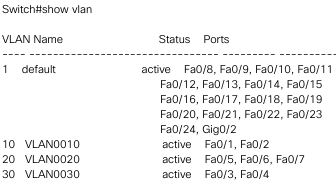
\includegraphics[width=0.8\textwidth]{images/scr01.png}
    \caption{Список виртуальных сетей на коммутаторе}
    \label{fig:vlan_database}
\end{figure}

\section{Задание 3}
В листинге \ref{lst:router} указаны команды, которые выполнялись для настройки моршрутизатора.
\begin{lstlisting}[frame=single,caption=Команды для настройки маршрутизатора,label=lst:router]
int gig0/0/0.1
encapsulation dot1q 10
ip address 192.168.14.254 255.255.255.0
exit
int gig0/0/0.2
encapsulation dot1q 20
ip address 192.168.15.254 255.255.255.0
exit
int gig0/0/0.3
encapsulation dot1q 30
ip address 192.168.16.254 255.255.255.0
exit
ip routing
\end{lstlisting}

В результате выполнения этих команд создались 3 подинтерфейса.

\section{Задание 4}
На рисунке \ref{fig:virt} выделены виртуальные сети.
\begin{figure}[H]
    \centering
    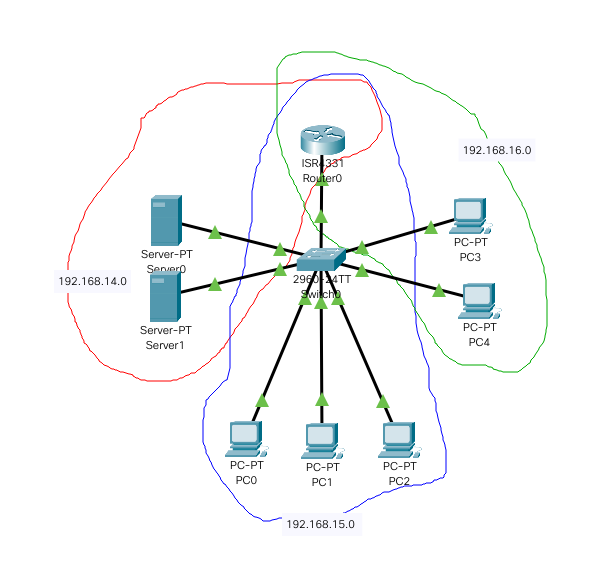
\includegraphics[width=0.8\linewidth]{images/scr02.png}
    \caption{Выделенные виртуальные сети}%
    \label{fig:virt}
\end{figure}

На рисунке \ref{fig:ping} представлен результат проверки соединения между Server0 и PC1.
\begin{figure}[H]
    \centering
    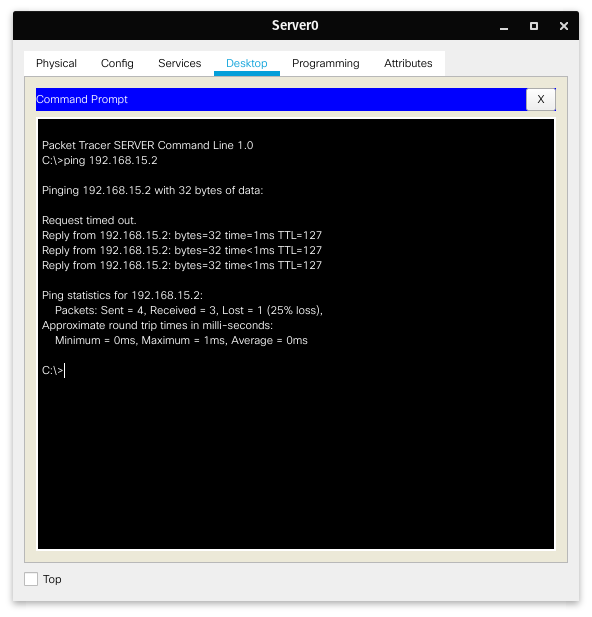
\includegraphics[width=0.5\linewidth]{images/scr03.png}
    \caption{Проверка соединения}%
    \label{fig:ping}
\end{figure}
